\section{Implementations}%
\label{sec:implementations}

\begin{frame}
	\frametitle{Getting into the computer}
	\framesubtitle{\url{https://xkcd.com/350}}

	\begin{center}
		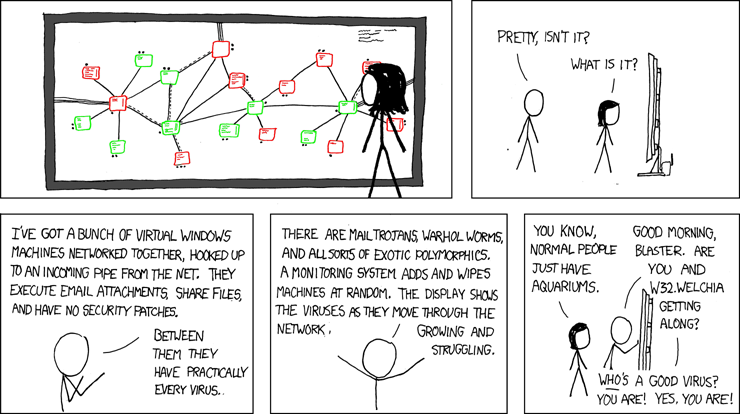
\includegraphics[width=0.8\textwidth]{figures/network.png}\\
	\end{center}
\end{frame}

\begin{frame}
	\frametitle{Implementing a graph}

	\begin{block}{Implementations}
		There are many options:
		\begin{itemize}
			\item Edge List: just keep one list of all edges of the graph.
				\pause
			\item Adjacency List: for every vertex, keep a list of all incident edges.
				\pause
			\item Adjacency Matrix: a massive 2D array of size $|V|\times |V|$. Every entry can hold an edge.
				\pause
			\item Adjacency Map: Just the best option. We will discuss this one now.
		\end{itemize}
	\end{block}	
\end{frame}

\begin{frame}
	\frametitle{Vertex class}
	
	\begin{columns}
		\column{0.505\textwidth}
			\lstinputlisting[basicstyle=\tiny\ttfamily, linebackgroundcolor={%
			\btLstHL<2>{3-5}%
			\btLstHL<3>{7-8}%
			\btLstHL<4>{10-11}%
			\btLstHL<5>{13-15}%
			\btLstHL<6>{17-23}%
			},
			lastline=23
			]{code/vertex.py}
		\column{0.455\textwidth}
		\begin{itemize}
			\pause
			\item Initialise a Vertex, with a \texttt{dict} to hold neighbours.
				\pause
			\item It is now $O(1)$ to add an edge, but this only works for \textit{simple} graphs.
				\pause
			\item Getting all neighbours is $O(\mathit{deg}(v))$, which is the best we can get.
				\pause
			\item A generator that allows us to iterate over the (outgoing) edges of this node.
				\pause
			\item And we can make more functions as need be.
		\end{itemize}
			
	\end{columns}
\end{frame}

\begin{frame}
	\frametitle{Graph class}
	
	\begin{columns}
		\column{0.505\textwidth}
			\lstinputlisting[basicstyle=\tiny\ttfamily, linebackgroundcolor={%
			\btLstHL<2>{3-4}%
			\btLstHL<3>{6-7}%
			\btLstHL<4>{9-10}%
			},
			lastline=10
			]{code/graph.py}
		\column{0.455\textwidth}
		\begin{itemize}
			\pause
			\item A graph is just a bunch of vertices now.
				\pause
			\item Adding a vertex is adding it to the dictionary.
			\item Using a dictionary allows $O(1)$ retrieval based on node name (e.g.\ Amsterdam)
				\pause
			\item Getting all vertices, is just all values from the list.
		\end{itemize}
			
	\end{columns}
\end{frame}

\begin{frame}
	\frametitle{Summary}

		\begin{exampleblock}{This implementation is awesome!}
			This implementation is better than all others (that you can find in the book), tomorrow we will see to what extent you can
			reproduce these ideas in the tutorial.
		\end{exampleblock}	

		\pause
		\begin{tabular}{c | c}
		Operation & Time complexity \\
		\midrule
		$|V|$ & $\Theta(1)$ \\
		$|E|$ & $\Theta(|V|)$\footnote{But we could make this $\Theta(1)$} \\
		\pause
		\texttt{degree(v)} & $\Theta(1)$ \\
		\texttt{neighbours(v)} & $\Theta(\mathit{deg}(v))$ \\
		\pause
		\texttt{add\_vertex(v)} & $\Theta(1)$ \\
		\texttt{add\_edge(v)} & $\Theta(1)$ \\
		\pause
		And a bunch more & See the book if you want\\
		\end{tabular}
\end{frame}
